% The mapping algorithm, step by step. Blue boxes call a language model; white boxes are code.
\definecolor{mdl}{HTML}{EAF2FB}\definecolor{mdld}{HTML}{2F6DB5}
\definecolor{cod}{HTML}{FFFFFF}\definecolor{codd}{HTML}{555555}
\definecolor{outp}{HTML}{E7F5EA}\definecolor{outpd}{HTML}{2E8B57}
\definecolor{giv}{HTML}{F3F3F3}\definecolor{humc}{HTML}{FDECEC}\definecolor{humcd}{HTML}{C0504D}
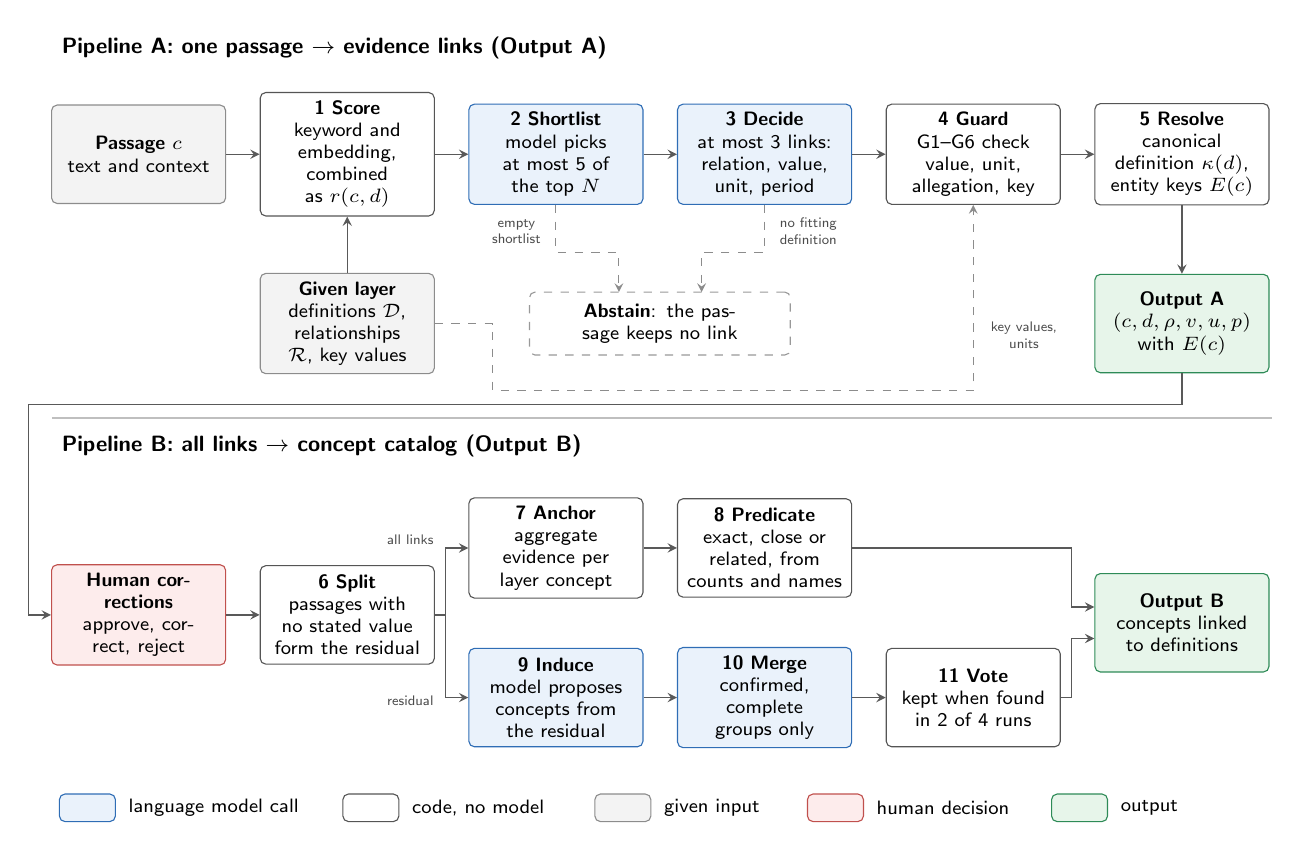
\begin{tikzpicture}[x=1cm,y=1cm,font=\sffamily\scriptsize,>=stealth,
  stp/.style={draw=codd,fill=cod,rounded corners=2pt,align=center,inner sep=3pt,minimum height=1.25cm,text width=2.0cm},
  model/.style={stp,draw=mdld,fill=mdl},
  given/.style={stp,draw=black!45,fill=giv},
  result/.style={stp,draw=outpd,fill=outp},
  human/.style={stp,draw=humcd,fill=humc,minimum height=0.8cm},
  arr/.style={->,line width=0.5pt,draw=black!65},
  quiet/.style={->,line width=0.4pt,draw=black!45,dashed},
  lab/.style={font=\sffamily\tiny,text=black!70,align=center}]
% ---------------- Pipeline A
\node[anchor=west,font=\sffamily\footnotesize\bfseries] at (0,9.55) {Pipeline A: one passage $\rightarrow$ evidence links (Output A)};
\node[given]  (pas) at (1.1,8.2)  {\textbf{Passage} $c$\\text and context};
\node[stp]   (sco) at (3.75,8.2) {\textbf{1 Score}\\keyword and embedding, combined as $r(c,d)$};
\node[model]  (sho) at (6.4,8.2)  {\textbf{2 Shortlist}\\model picks at most 5 of the top $N$};
\node[model]  (dec) at (9.05,8.2) {\textbf{3 Decide}\\at most 3 links: relation, value, unit, period};
\node[stp]   (gua) at (11.7,8.2) {\textbf{4 Guard}\\G1--G6 check value, unit, allegation, key};
\node[stp]   (key) at (14.35,8.2){\textbf{5 Resolve}\\canonical definition $\kappa(d)$, entity keys $E(c)$};
\node[result] (oa)  at (14.35,6.05){\textbf{Output A}\\$(c,d,\rho,v,u,p)$ with $E(c)$};
\node[given]  (lay) at (3.75,6.05){\textbf{Given layer}\\definitions $\mathcal{D}$, relationships $\mathcal{R}$, key values};
\node[stp,draw=black!40,dashed,text width=3.1cm,minimum height=0.8cm] (abs) at (7.72,6.05) {\textbf{Abstain}: the passage keeps no link};
\draw[arr] (pas) -- (sco); \draw[arr] (sco) -- (sho); \draw[arr] (sho) -- (dec);
\draw[arr] (dec) -- (gua); \draw[arr] (gua) -- (key); \draw[arr] (key) -- (oa);
\draw[arr] (lay) -- (sco);
\draw[quiet] (sho.south) -- (6.4,6.95) -- (7.2,6.95) -- (7.2,6.45);
\draw[quiet] (dec.south) -- (9.05,6.95) -- (8.25,6.95) -- (8.25,6.45);
\node[lab,anchor=east] at (6.33,7.22) {empty\\shortlist};
\node[lab,anchor=west] at (9.12,7.22) {no fitting\\definition};
\draw[quiet] (lay.east) -- (5.6,6.05) -- (5.6,5.2) -- (11.7,5.2) -- (gua.south);
\node[lab,anchor=west] at (11.8,5.9) {key values,\\units};
% ---------------- Pipeline B
\draw[black!25,line width=0.4pt] (0,4.85) -- (15.5,4.85);
\node[anchor=west,font=\sffamily\footnotesize\bfseries] at (0,4.5) {Pipeline B: all links $\rightarrow$ concept catalog (Output B)};
\node[human]  (cor) at (1.1,2.35)  {\textbf{Human corrections}\\approve, correct, reject};
\node[stp]   (spl) at (3.75,2.35) {\textbf{6 Split}\\passages with no stated value form the residual};
\node[stp]   (anc) at (6.4,3.2)  {\textbf{7 Anchor}\\aggregate evidence per layer concept};
\node[stp]   (pre) at (9.05,3.2) {\textbf{8 Predicate}\\exact, close or related, from counts and names};
\node[model]  (ind) at (6.4,1.3) {\textbf{9 Induce}\\model proposes concepts from the residual};
\node[model]  (mer) at (9.05,1.3){\textbf{10 Merge}\\confirmed, complete groups only};
\node[stp]   (vot) at (11.7,1.3){\textbf{11 Vote}\\kept when found in 2 of 4 runs};
\node[result] (ob)  at (14.35,2.25){\textbf{Output B}\\concepts linked to definitions};
\draw[arr] (oa.south) -- (14.35,5.02) -- (-0.3,5.02) -- (-0.3,2.35) -- (cor.west);
\draw[arr] (cor) -- (spl);
\draw[arr] (spl.east) -- (5.0,2.35) -- (5.0,3.2) -- (anc.west);
\draw[arr] (spl.east) -- (5.0,2.35) -- (5.0,1.3) -- (ind.west);
\node[lab,anchor=south east] at (4.97,3.12) {all links};
\node[lab,anchor=north east] at (4.97,1.45) {residual};
\draw[arr] (anc) -- (pre); \draw[arr] (ind) -- (mer); \draw[arr] (mer) -- (vot);
\draw[arr] (pre.east) -- (12.95,3.2) -- (12.95,2.45) -- (ob.west|-0,2.45);
\draw[arr] (vot.east) -- (12.95,1.3) -- (12.95,2.05) -- (ob.west|-0,2.05);
% ---------------- legend
\node[model,minimum height=0.35cm,text width=0.5cm] at (0.45,-0.1) {};
\node[anchor=west] at (0.85,-0.1) {language model call};
\node[stp,minimum height=0.35cm,text width=0.5cm] at (4.05,-0.1) {};
\node[anchor=west] at (4.45,-0.1) {code, no model};
\node[given,minimum height=0.35cm,text width=0.5cm] at (7.25,-0.1) {};
\node[anchor=west] at (7.65,-0.1) {given input};
\node[human,minimum height=0.35cm,text width=0.5cm] at (9.95,-0.1) {};
\node[anchor=west] at (10.35,-0.1) {human decision};
\node[result,minimum height=0.35cm,text width=0.5cm] at (13.05,-0.1) {};
\node[anchor=west] at (13.45,-0.1) {output};
\end{tikzpicture}
